%
% Szablon, v. 3.0
% p.wlaz@pollub.pl
%

% PROSZĘ NIE USUWAĆ
% KOMENTARZY Z~PREAMBUŁY
% JEŻELI KTOŚ WAM WMAWIA, ŻE
% TO PRZYSPIESZY COKOLWIEK
% -- MYLI SIĘ!


\documentclass[12pt]{mwbk}


%%%%%%% marinesy, rozmiary, to warto dopasować do drukarki
\usepackage[a4paper,twoside,top=2.6cm,bottom=2.6cm,inner=3cm,outer=2.6cm]{geometry}

%%%%%%%% polszczyzna
\usepackage[T1]{polski}


%%%%%%%%% sposób kodowania literek w edytorze
\usepackage[utf8]{inputenc}

\usepackage[font=small,labelfont=bf,justification=centering]{caption}


%%%% gdyby ktoś chciał powyklejać z~pedeefa
%%%% teksty za pomocą AcroReadera, to 
%%%% poniższe dwie linijki pomogą w~tym
%%%% Może to być przydatne, gdyby ktoś na podstawie
%%%% elektronicznej wersji chciał przygotować dane do 
%%%% badania antyplagiatowego
%%%% ponieważ prace są w
%%%% tych czasach różnymi
%%%% programami antyplagiatowymi
%%%% proszę absolutni NIE
%%%% USUWAĆ następujących
%%%% dwu linijek
\input glyphtounicode.tex
\pdfgentounicode = 1

%%%%%%%%%%%%%%%%%%%%%%%%%%%%%%%%%%%%%
%%%%% jeśli chcesz by główny tekst oraz wzory matematyczne były
%%%%% składane czcionką typu Times Roman (w~odróżnieniu od standardowej
%%%%% TeXowej, czyli Computer Modern Roman) to linia poniżej
%%%%% ma być 'aktywna', następna nieaktywna, 
%%%%% jeśli zrobisz odwrotnie (pierwsza nieaktywna,
%%%%% druga aktywna) uzyskasz skład czcionką
%%%%% Computer Modern Roman mającą wielu wiernych
%%%%% fanów w~świecie TeXa). Konsekwencją jednak będą zmiany
%%%%% rozmiarów czcionek dla rozdziałó i podrozdziałów - rzecz bez większego
%%%%% znaczenia, wynikająca z pewnych zaszłości historycznych (ComputerModern
%%%%% niegdyś były używane wyłącznie w postaci tzw. bitmap)
\usepackage{mathptmx} \usepackage{tgtermes}
%\usepackage{lmodern}

%%% WSZELKIE ZMIANY W~PREAMBULE RÓB ROZWAŻNIE
%%% NIE JESTEŚ PEWNY/PEWNA ICH EFEKTU TO~SPRAWDŹ 
%%% CZY W~PRGRAMIE ADOBE READER (i~to dokładnie
%%% o~ten program chodzi, nie o~jakikolwiek)
%%% Z~WYNIKOWEGO PLIU PDF DA SIE PRAWIDŁOWO
%%% WYKLEIĆ TEKST Z~POLSKIMI LITERAMI, BEZ KRZAKÓW,
%%%% BEZ DZIWACTW.


%%%%%%%%%%%%%% pozostałe pakiety używane w~pracy, to już zależy od
%%%%%%%%%%%%%% autora, więc może być tego więcej
\usepackage{fancyhdr}
\usepackage{graphicx}
\usepackage{amsmath}
\usepackage{amsthm}
\usepackage{amssymb}
\usepackage{url}
\usepackage{longtable}
\usepackage{array,hhline}

%%%%%%%% hyperref po to by przeglądarka pedeef ukazywala na odwołania
%%%%%%%% prawidłowo skonstruowane za pomocą \ref, \cite i.t.d. jako
%%%%%%%% hiperłącza
\usepackage{hyperref}



%%%%% dla fanów ``profesjonalnych'' tabel w~stylu zachodnich książek

\usepackage{booktabs} \heavyrulewidth=1.5bp \lightrulewidth=0.5bp


%%%%%%%%%%% poniżej uniwersalny sposób na ucywilizowanie znaków 
%%%%%%%%%%% niewiększości, niezależny od pakietu {polski}, ale za to 
%%%%%%%%%%% zależny od {amssymb}, ma tą zaletę, że działa np. z Timesem
%%%%%%%%%%% w matematyce
\let\leq\leqslant\let\le\leq\let\geq\geqslant\let\ge\geq


%%%%%%% jeżeli będziesz chciał włączać do swojej pracy fragmenty programów, 
%% to ponizsza linijka przyda się, jeśli nie - usuń ją

\usepackage{fancyvrb}


%%%%%%%%%%%%%%%%% struktury do tworzenia twierdzeń i~tym podobnych

\theoremstyle{plain}
\newtheorem{twier}{Twierdzenie}[chapter] % pierwsze to nazwa środowiska,
                                      %drugie to wyświetlana nazwa
				% to trzecie w~nawiasie kwadratowym
				% wskazuje numer dolepiony z~lewej do
				% numeru twierdzenia (tu numer
				% 'chapter', 
\newtheorem{lemat}{Lemat}[chapter]

\theoremstyle{definition}
\newtheorem{defi}{Definicja}[chapter]

\theoremstyle{remark}
\newtheorem{uwaga}{Uwaga}[chapter]
\newtheorem{wniosek}{Wniosek}[chapter]

%%%%% więcej możliwości w~dokumentacji amsthm



%%%%%%%%%%%%%%%%%%%%%%%%%%%%%%%%%%%%%%%%%5
%%%%%%%%%%%%%%%%%%%%%%%%%%%%%%%%%%%%%%%%%%
%%%%%%%%% wcięcie akapitowe %%%%%%%%%%%%%%
%%%%%%%%%%%%%%%%%%%%%%%%%%%%%%%%%%%%%%%%%%
%%%%%% ustawić w~zaleceń i~gustu %%%%%%%%%
%%%%%%%%%%%%%%%%%%%%%%%%%%%%%%%%%%%%%%%%%%
%%%%%%%% zalecenie na stronie wydziałowej
%%%%%%%% było 1.25cm i wyglądało jakoś 
%%%%%%%% śmiesznie duże, więc spłoszony nieco
%%%%%%%% wpisałem 1cm, ale uważny czytelnik już
%%%%%%%% zapewne się domyśli, że podmiana napisu 
%%%%%%%% =1cm na =1.25cm sprawi, że wcięcia na początku
%%%%%%%% akapitu ustawią się na (nieco przydużą)
%%%%%%%% wartość 1.25cm 

\parindent=1cm



%%%%%%%%%%%%%%%%%%%%%%%%%%%%%%%%
%%%%% tu pewne poluzowanie rozmieszczenia elementów tabelek
%%%%% możecie sobie poeksperymentować, by dopasować do swych
%%%%% gustów, a przede wszystkim gustów promotorów (promotorek)
  \tabcolsep=4mm          
  %\renewcommand\arraystretch{1.3}
%%%%%%%%%%%%%%%%%%%%%%%%%%%%%%%%%%



%%%%%%%%% teraz żywa pagina (aka 'running headline') i~numerowanie stron
%%%%%%%%%%%%%%%%%%%%%%%%%%%%%%%%%%%%%%%%%%%%%%%%%%%%%%%%%%%%%%%%%%%%%%%%
%%%%%na górze mają być śródtytuły, na dole (po stronie zewneętrznej)
%%%%%numery stron. Poszedłem kapkę dalej i~na stronach ropoczynających
%%%%%rozdział nie ma paginy (górki).
%%%%% Oczywiście jeśli ostatnia strona
%%%%% jest pusta (uzupełnia jeno parzystość) to tam żadnej stopki ani 
%%%%% górki byc mnie może - ma być pusta.
%%%%%%%%%%%%%%%%%%%%%%%%%%%%
\pagestyle{fancy}
\fancyhead{}% oczyszczenie
\fancyhead[RO]{\rightmark} %% na nieparzystych 'podległe' śródtytuły
\fancyhead[LE]{\leftmark} %% na parzystych 'ważniejsze'
\fancyfoot{}% oczyszczenie
\fancyfoot[RO,LE]{\arabic{page}}  %% numer na dole (po prawej na
%% nieparzystych, po lewej na parzystych)
\renewcommand\headrulewidth{0.4pt} %%% cienka hrulka oddzielająca paginę
                                    %%% od kolumny tekstu
\fancypagestyle{closing}{%%%%%% to styl dla stron zamykających rozdział
\fancyhead{}% oczyszczenie
\fancyhead[RO]{\rightmark} %% na nieparzystych 'podległe'
\fancyhead[LE]{\leftmark} %% na parzystych 'ważniejsze'
\fancyfoot{}% oczyszczenie
\fancyfoot[RO,LE]{\arabic{page}}  %% numer na dole (po prawej na
                                  %% powyższą linijkę usuń jeśli nie
				  %% chcesz numerów na niepełnych
				  %% kolumnach (zamykających rozdział)
\renewcommand\headrulewidth{0.4pt}
}
\fancypagestyle{opening}{%%% styl stron rozpoczynających rozdział
\fancyhead{}% oczyszczenie
\fancyfoot{}% oczyszczenie
\fancyfoot[RO,LE]{\arabic{page}}  %% numer na dole (po prawej na
\renewcommand\headrulewidth{0pt}
}
\fancypagestyle{plain}{%%%% styl zwykły, niektóre konstrukcje
                       %%%% (typu \titlepage, którego ja tu nie używam
                       %%%% ale może są jakieś inne o których nawet nie chce 
                       %%% mi się myśleć, więc dla spokoju robię to po swojemu
\fancyhead{}% oczyszczenie
\fancyfoot{}% oczyszczenie
\fancyfoot[RO,LE]{\arabic{page}}  %% numer na dole (po prawej na
\renewcommand\headrulewidth{0pt}
}

%%%%%%%%%%%%%%%%%%%%%%%%%%%%%%%%%5
%%%%%%%%%%%%%%%%%%%%%%%%%%%%%%%%%%
%%% lekka modyfikcja 'markow' do paginy
%%% uznalem, ze jesli ktos nie da \section (np we wstepnie czy
%%% podsumowaniu to niech na obu sronach w~paginie pojawia sie tytuł
%%% chaptera, bo standardowo, to na nieparzystej stronie w takiej sytuacji
%%% nad górną linią ziałaby pustka, co mogłoby wprowadzać konsternację
\makeatletter
    \def\chaptermark#1{%
      \markboth{%
        \ifHeadingNumbered
     \if@mainmatter
     \@chapapp\
            \thechapter.\enspace
          \fi
        \fi
        #1}{%
        \ifHeadingNumbered
     \if@mainmatter
     \@chapapp\
            \thechapter.\enspace
          \fi
        \fi
        #1%
	}}%
    \def\sectionmark#1{%
      \markright{%
        \ifHeadingNumbered \thesection.\enspace \fi
        #1}}
%%%%%%%%%%%%%%%%%%%%%%%%%%%%%%%%%%%%%%%%%%%%%%%
%%%%%%%%%%%%%%%%%%%%%%%%%%%%%%%%%%%%%%%%%%%%%%%%
%%%%%%%%%%%% wielkości czcionek dla chapter i~section
%%%%%%%%%%%% 16 dla rozdziału, 14 dla podrozdziału - te domyślne
%%%%%%%%%%%% w klasie mwbk były całkiem ładne, ale żeby nie było
%%%%%%%%%%%% że nie potrafię ustawić
%%%%%%%%%%%%%%%%%%%%%%%%%%%%%%%%%%%%%%%%%%%%%%%%%%%
\SetSectionFormatting[breakbefore,wholewidth]{chapter}
        {0\p@}
        {\FormatRigidChapterHeading{6.4\baselineskip}{12\p@}%
	{\large\@chapapp\space}{\fontsize{16}{19}\selectfont}}
        {1.6\baselineskip}
\SetSectionFormatting{section}
        {24\p@\@plus5\p@\@minus2\p@}
	{\FormatHangHeading{\fontsize{14}{16}\selectfont}}
        {10\p@\@plus3\p@}
\makeatother	



%%%%%%%%%%%%%%%%%%%%%%%%%%%%%%%%%%%%%%%%%%%%%%
%%%%%%%%%%%%%%%%%%%%%%%%%%%%%%%%%%%%%%%%%%%%%%
%%%%%%%%%%%%%% jakies inne pomocnicze definicje, ja na przykład lubię
% \R
%%%%%%%%%%%%%%%%%%%%%%%5
%%%%%%%%%%%%%%%%%%%%%%%
%%%% tak naprawdę są t potrzebne tylko po to
%%%% by zadziałały przykłady poniżej w tekście
%%%% które w sposób dość losowy zostały 
%%%% pobrane z jakichś moich starych plików
%%%%%%%%%%%%%%%%%%%%%%%%%%%%%%%%%%
%%%%%%%%%%%%%%%%%%%%%%%%%%%%%%%%%%%
%%%% w realnej pracy te poniższe śmieci możecie oczywiście
%%%% usunąć
%%%%%%%%%%%%%%%%%%%%%%%%%%%%
\newcommand\R{\mathbb{R}}
\newcommand{\ff}{\mathbf{f}}
\newcommand{\hh}{\mathbf{h}}
\newcommand{\xx}{\mathbf{x}}
\newcommand{\yy}{\mathbf{y}}
\newcommand{\zz}{\mathbf{z}}
\newcommand{\gggg}{\mathbf{g}}
\newcommand{\skalar}[2]{\pmb{\langle}#1,#2\pmb{\rangle}}
%%%%%%%%%%%% koniec tych dodatkowych definicji

%%%%%% trocę więcej ``luzu'' przy rozmieszczaniu {fgur} i~{table}

 \renewcommand{\topfraction}{0.9}	% max fraction of floats at top
    \renewcommand{\bottomfraction}{0.8}	% max fraction of floats at bottom
    %   Parameters for TEXT pages (not float pages):
    \setcounter{topnumber}{2}
    \setcounter{bottomnumber}{2}
    \setcounter{totalnumber}{4}     % 2 may work better
    \setcounter{dbltopnumber}{2}    % for 2-column pages
    \renewcommand{\dbltopfraction}{0.9}	% fit big float above 2-col. text
    \renewcommand{\textfraction}{0.07}	% allow minimal text w. figs
    %   Parameters for FLOAT pages (not text pages):
    \renewcommand{\floatpagefraction}{0.7}	% require fuller float pages
    % N.B.: floatpagefraction MUST be less than topfraction !!
    \renewcommand{\dblfloatpagefraction}{0.7}	% require fuller float pages
    % remember to use [htp] or [htpb] for placement

    
%%% DWA proste polecenia służące do ujednolicenia podawania źródeł przy rysunkach i~tabelkach    
    
    \newcommand\zrodlo[1]{\par\vspace{-3mm}{\small\textit{Źródło: }#1 }}
    \newcommand\zrodlotab[1]{{\par\vspace{2mm}\small\textit{Źródło: }#1 }}

\raggedbottom   %%% to znaczy, że nie będzie siłowego wyrównywania typowych
                %%     stron do jednakowej wysokości

\linespread{1.3}
\begin{document}

%%%%%%%%%%%%%%%%%%%%%%%%%%%%%%%%%%%%%%%%%
%%%%%%%%%%%%%%%%%%%%%%%%%%%%%%%%%%%%%%%%%
%%%%%%%% STRONA TYTUŁOWA %%%%%%%%%%%%%%%%

\thispagestyle{empty}  % tu wszak nie chcemy żadnej numeracji stron


%%%%%%%%%%%%%%%%%%%%%%%%%%%%%%%%%%%%%%%%%%%%%%%%%%%%%%%%%%%%%%%
%%%%%tytuły definiuje jako makrodefinicje, gdyż zamierzam je%%%
%%%%%powtórzyć na stronie ze streszczeniami, to nic nie boli%%%
%%%%%a gwarantuje, że będą one takie same, i~tak ma być.%%%%%%%
%%%%%%%%%%%%%%%%%%%%%%%%%%%%%%%%%%%%%%%%%%%%%%%%%%%%%%%%%%%%%%%
\newcommand\tytul{Przegląd autoenkoderów stosowanych w nienadzorowanym uczeniu maszynowym}

\newcommand\tytulangielski{An overview of autoencoders used in unsupervised machine learning}



\noindent\hspace{-32pt}
\includegraphics{rys/logopl}
\begin{center}
	



%%{\large \bf POLITECHNIKA LUBELSKA}

%%%% {\bf WYDZIAŁ PODSTAW TECHNIKI} tego już nie chcą w~nowym wzorcu karty

%%%% \emph{Kierunek:} MATEMATYKA   %% już jest w~``logo''

%%% BEZ SPEC.!!! \emph{Specjalność:} Matematyka w~finansach i~ubezpieczeniach

\vfill %%%% \vfill to taki rozpychacz w pionie, pcha ile mu pozwolą
     


\vfill

\textbf{Praca magisterska}

\vfill
\vfill
\vfill

\large
\tytul

\vfill

\emph{\tytulangielski}


\vfill
\vfill
\vfill
\vfill
\vfill

\begin{tabular}[t]{l}
\emph{Praca wykonana pod kierunkiem:}
\\
dra Dariusza Majerka
\end{tabular}
\hfill
\begin{tabular}[t]{l}
	\emph{Autor:}
\\
Alicja Hołowiecka\\
nr albumu: 89892 
\end{tabular}

\vfill
\vfill
\vfill

\textbf{Lublin 2022}

\end{center}


%%%%% koniec tytułów


%%%%%%%%%%%%%%%%%%%%%%%5
%%%%%%%%%%%%%%%%%%%%%%
%%% teraz spis treści
%%%%%%%%%%%%%%%%%%%%%
%%% pamiętaj! po jakiejkolwiek zmianie w tekście
%%% która wpływa na zmianę spisu treści, spis będzie dobry co najmniej
%%% po dwóch przebiegach latexa - to samo dotyczy odwołań do wzorów i literatury
%%% ogólnie to przed wydrukiem warto przelatexować o jedne raz więcej niż
%%% to się wydaje konieczne, no chyba że korzystamy z funkcji typu BUILD
%%% w zintegrowanym systemie wspomagającym TeX, BUILD powinien takie sprawy 
%%% wziąć pod uwagę

\tableofcontents


\chapter*{Wstęp}



\chapter{Przegląd autoenkoderów}

\section{Sztuczne sieci neuronowe}

\textbf{Sztuczny neuron} ma co najmniej jedno binarne wejście i dokładnie jedno binarne wyjście. Wyjście jest uaktywniane, jeżeli jest aktywna określona liczba wejść. Na rysunku \ref{fig:neurony1} przedstawione są przykładowe sztuczne sieci neuronowe (SSN lub z angielskiego ANN) wykonujące różne operacje logiczne, przy założeniu, że neuron uaktywni się, gdy przynajmniej dwa wejścia będą aktywne \cite{geron}.

\begin{figure}[!h]
	\centering
	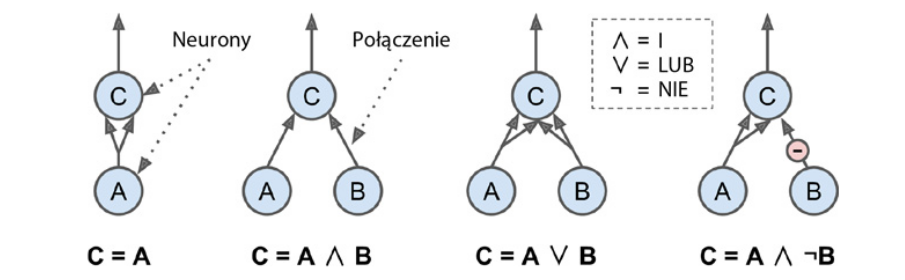
\includegraphics[width=9cm]{rys/neurony1.png}
	\caption{Przykładowe sztuczne sieci neuronowe rozwiązujące proste zadania logiczne}
	\zrodlo{\cite{geron}}
	\label{fig:neurony1}
\end{figure}

Jedną z najprostszych architektur SSN jest \textbf{perceptron}, którego podstawą jest sztuczny neuron zwany \textbf{progową jednostką logiczną} (ang. \textit{Threshold Logic Unit} - TLU) lub \textbf{liniową jednostką progową} (ang. \textit{Linear Threshold Unit} - LTU). Wartościami wejść i wyjść są liczby, a każde połączenie ma przyporządkowaną wagę. Jednostka TLU oblicza ważoną sumę sygnałów wejściowych, a następnie zostaje użyta funkcja skokowa. Schemat takiej jednostki został przedstawiony na rysunku \ref{fig:neurony2}.

\begin{figure}[!h]
	\centering
	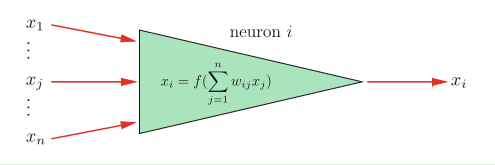
\includegraphics[width=8cm]{rys/neurony2.png}
	\caption{Struktura sztucznego neuronu, który stosuje funkcję skokową $f$ na ważonej sumie sygnałów wejściowych}
	\zrodlo{\cite{ertel}}
	\label{fig:neurony2}
\end{figure}

Często używaną funkcją skokową jest \textbf{funkcja Heaviside'a}, określona równaniem 

$$H(z)=\begin{cases}
0, & \text{ jeśli } z<0\\
1, & \text{ jeśli } z \geq 0
\end{cases}$$

Czasami stosuje się również \textbf{funkcję signum}

$$sgn(z)=\begin{cases}
-1 & \text{ jeśli } z<0\\
0, & \text{ jeśli } z=0\\
1, & \text{ jeśli } z > 0
\end{cases}$$

Perceptron jest złożony z jednej warstwy jednostek TLU, w której każdy neuron jest połączony ze wszystkimi wejściami. Tego typu warstwa jest nazywana \textbf{warstwą gęstą}. Warstwa, do której są dostarczane dane wejściowe, jest nazywana \textbf{warstwą wejściową} (ang. \textit{input layer}). Najczęściej do tej warstwy jest wstawiany również \textbf{neuron obciążeniowy} (ang. \textit{bias neuron}) $x_0=1$, który zawsze wysyła wartość 1. Na rysunku \ref{fig:perceptron1} znajduje się perceptron z dwoma neuronami wejściowymi i jednym obciążeniowym, a także z trzema neuronami w warstwie wyjściowej.

\begin{figure}[!h]
	\centering
	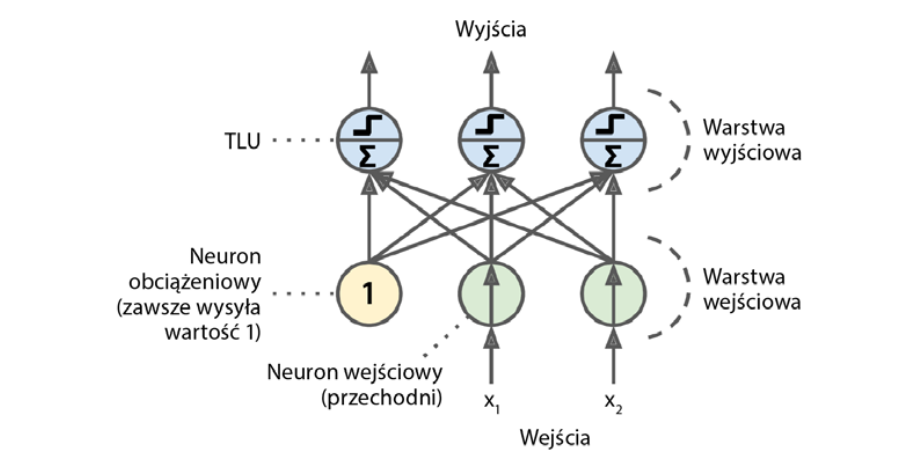
\includegraphics[width=10cm]{rys/perceptron1.png}
	\caption{Perceptron z trzema neuronami wejściowymi i trzema wyjściami}
	\zrodlo{\cite{geron}}
	\label{fig:perceptron1}
\end{figure}

Obliczanie sygnałów wyjściowych w warstwie gęstej przedstawia się wzorem
$$h_{\mathbf{W},\mathbf{b}}(\mathbf{X})=\phi(\mathbf{XW}+\mathbf{b})$$
gdzie $\mathbf{X}$ - macierz cech wejściowych, $\mathbf{W}$ - macierz wag połączeń (oprócz neuronu obciążeniowego), $\mathbf{b}$ - wektor obciążeń zawierający wagi połączeń neuronu obciążeniowego ze wszystkimi innymi neuronami, $\phi$ - tzw. \textbf{funkcja aktywacji}, w przypadku TLU jest to funkcja skokowa.

Algorytm uczący, który służy do trenowania perceptronu, jest silnie inspirowany działaniem neuronu biologicznego. Gdy biologiczny neuron często pobudza inną komórkę nerwową, to połączenia między nimi stają się silniejsze. Reguła ta jest nazywana \textbf{regułą Hebba}. Perceptrony są uczone za pomocą odmiany tej reguły, w której połączenia są wzmacniane, jeśli pomagają zmniejszyć wartość błędu. Dokładniej, w danym momencie perceptron przetwarza jeden przykład uczący i wylicza dla niego predykcję. Na każdy neuron wyjściowy odpowiadający za nieprawidłową prognozę następuje zwiększenie wag połączeń ze wszystkimi wejściami przyczyniającymi się do właściwej prognozy. Aktualizowanie wag przedstawia się następującym wzorem
$$\Delta w_{ij}=\eta (y_j-\hat{y_j})x_i$$
gdzie $w_{ij}$ - waga połączenia między $i$-tym neuronem wejściowym a $j$-tym neuronem wyjściowym, $x_i$ - $i$-ta wartość wejściowa bieżącego przykładu uczącego, $\hat{y_j}$ - wynik $j$-tego neuronu wyjściowego dla bieżącego przykładu uczącego, $y_j$ - docelowy wynik $j$-tego neuronu, $\eta$ - współczynnik uczenia.

Perceptron ma wiele wad związanych z niemożnością rozwiązania pewnych trywialnych problemów (np. zadanie klasyfikacji rozłącznej czyli XOR). Część tych ograniczeń można wyeliminować, stosując architekturę SSN złożoną z wielu warstw perceptronów, czyli \textbf{perceptron wielowarstwowy} (ang. \emph{Multi-Layer Perceptron}). Składa się on z jednej warstwy wejściowej (przechodniej), co najmniej jednej warstwy jednostek TLU - tzw. \textbf{warstwy ukryte} (ang. \emph{latent layers}) i ostatniej warstwy jednostek TLU - warstwy wyjściowej. Oprócz warstwy wejściowej każda warstwa zawiera neuron obciążający i jest w pełni połączona z następną wartswą. Sieć zawierająca wiele warstw ukrytych nazywamy \textbf{głęboką siecią neuronową} (ang. \emph{Deep Neural Network} - DNN). 

Do uczenia perceptronów wielowarstwowych wykorzystywany jest algorytm \textbf{propagacji wstecznej} (ang. \emph{backpropagation}). Propagacja wsteczna jest właściwie algorytmem gradientu prostego \cite{skansi}. Można go zapisać jako
$$w_{updated}=w_{old}-\eta \nabla E$$
gdzie $E$ jest funkcją kosztu (funkcją straty) \cite{skansi}. Proces jest powtarzany do momentu uzyskania zbieżności z rozwiązaniem, a każdy przebieg jest nazywany \textbf{epoką} (ang. \emph{epoch}).

\begin{uwaga}
	Wagi połączeń wszystkich warstw ukrytych należy koniecznie zainicjować losowo. W przeciwnym przypadku proces uczenia zakończy się niepowodzeniem. Na przykład jeśli wszystkie wagi i obciążenia zostaną zainicjowane wartością 0, to model będzie działał tak, jak gdyby składał się tylko z jednego neuronu. Przy zainicjowaniu wag losowo, symetria zostanie złamana i algorytm propagacji wstecznej będzie w stanie wytrenować zespół zróżnicowanych neuronów \cite{geron}. 
\end{uwaga}

Aby algorytm propagacji wstecznej działał prawidłowo, kluczową zmianą jest zastąpienie funkcji skokowej przez inne \textbf{funkcje aktywacji}. Zmiana ta jest konieczna, ponieważ funkcja skokowa zawiera jedynie płaskie segmenty i przez to nie pozwala korzystać z gradientu. 

Najczęściej używana jest \textbf{funkcja logistyczna (sigmoidalna)}
$$\sigma(z)=\frac{1}{1+e^{-z}}$$
Ma ona w każdym punkcie zdefiniowaną pochodną niezerową, dzięki czemu algorytm gradientu prostego może na każdym etapie uzyskać lepsze wyniki. Zbiór wartości tej funkcji wynosi od 0 do 1.

Inną popularną funkcją aktywacji jest \textbf{tangens hiperboliczny}
$$\operatorname{tanh}(z)=2\sigma(2z)-1$$
Funkcja ta jest ciągła i różniczkowalna, a jej zakres wartości wynosi $-1$ do 1. Dzięki temu zakresowi wartości wynik każdej warstwy jest wyśrodkowany wobec zera na początku uczenia, co często pomaga w szybszym uzyskaniu zbieżności.

Wśród popularnych funkcji aktywacji należy także wyróżnić  \textbf{funkcję ReLU} (ang. \emph{Rectified Linear Unit} - prostowana jednostka liniowa) o wzorze
$$ReLU(z)=max(0,z).$$
Jest ona ciągła, ale nieróżniczkowalna w punkcie 0. Jej pochodna dla $z<0$ wynosi zero. Jej atutem jest szybkość przetwarzania. Nie ma ona maksymalnej wartości wyjściowej.
W zadaniach regresji bywa wykorzystywany ,,wygładzony'' wariant funkcji ReLU, czyli funkcja \textbf{softplus}:
$$softplus(z)=log(1+exp(z))$$

Na  rysunku \ref{fig:funkcje-aktywacji} przedstawiono popularne funkcje aktywacji wraz z ich pochodnymi.

\begin{figure}[!h]
	\centering
	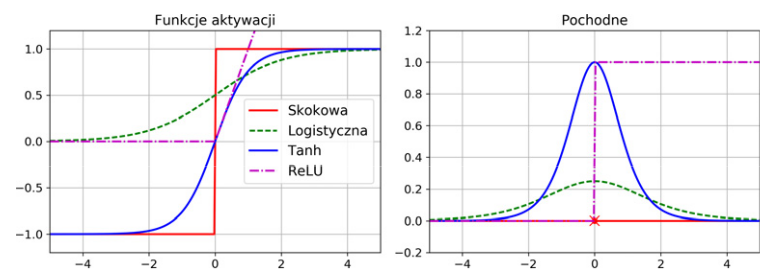
\includegraphics[width=\linewidth]{rys/funkcje_aktywacji.png}
	\caption{Przykładowe funkcje aktywacji wraz z pochodnymi}
	\zrodlo{\cite{geron}}
	\label{fig:funkcje-aktywacji}
\end{figure}

\section{Sieci splotowe}

Sieci splotowe, nazywane również \textbf{splotowymi sieciami neuronowymi} (ang. \emph{convolutional neural networks}, CNN), są rodzajem sieci neuronowych służących do przetwarzania danych o znanej topologii siatki. Przykładem takich danych są szeregi czasowe, które można uznać za jednowymiarową siatkę z próbkami w regularnych odstępach czasu, oraz dane graficzne, które można interpretować jako dwuwymiarową siatkę pikseli. Nazwa sieci splotowych pochodzi od wykorzystywanego przez te sieci działania matematycznego nazywanego \textbf{splotem} (konwolucją). Można powiedzieć, że sieci splotowe to po prostu sieci neuronowe, które w przynajmniej jednej z warstw zamiast ogólnego mnożenia macierzy wykorzystują splot \cite{goodfellow}.


\cite{geron}

Splotowe sieci neuronowe stanowią wynik badań nad korą wzrokową. Są używane głównie do rozpoznawania obrazów (od lat 80-tych XX w.).

Zagadnienia rozpoznawania obrazu:
\begin{itemize}
	\item klasyfikacja
	\item detekcja obrazów
	\item transfer stylu
\end{itemize}

Neurony biologiczne w korze wzrokowej reagują na określone wzorce w niewielkich obszarach pola wzrokowego, zwanych polami recepcyjnymi; w miarę przepływu sygnału wzrokowego przez kolejne moduły w mózgu neurony rozpoznają coraz bardziej skomplikowane wzorce wykrywane w coraz większych polach recepcyjnych.

Wiele neuronów tworzących korę wzrokową tworzą lokalne pola recepcyjne, reagujące jedynie na bodźce wzrokowe mieszczące się w określonym rejonie pola wzrokowego.

Pola recepcyjne poszczególnych neuronów mogą się na siebie nakładać.

Pola recepcyjne łącznie tworzą całe pole wzrokowe.

Pewne neurony reagują wyłącznie na obrazy składające się z linii poziomych, lub innych linii ułożonych w konkretny sposób.

Niektóre komórki nerwowe mają większe pola recepcyjne i wykrywają bardziej skomplikowane kształty.

Neurony odpowiedzialne za rozpoznawanie bardziej skomplikowanych kształtów znajdują się na wyjściu neuronów reagujących na prostsze bodźce.


\subsection{Hiperparametry filtru konwolucyjnego}

\cite{illustrated}

Warstwy konwolucyjne w przeciwieństwie do zagęszczonych, nie są w pełni połączone. Oznacza to, że w pierwszej warstwie ukrytej nie są wiązane wagi wszystkich pikseli ze wszystkimi neuronami. Zamiast tego stosowanych jest kilka wymienionych niżej hiperparametrów określających liczbę wag i odchyleń związanych z daną warstwą konwolucyjną:
\begin{itemize}
	\item wielkość jądra (kernel size) - jądro (zwane również filtrem lub polem receptywnym) typowo ma wysokość i szerokość trzech pikseli. Rozmiar ten okazał się optymalny w szerokim zakresie zastosowań widzenia maszynowego w nowoczesnych sieciach konwolucyjnych. Popularna jest również wielkość 5x5 pikseli, a maksymalny stosowany rozmiar to 7x7 pikseli. Jeśli jądro jest zbyt duże w stosunku do obrazu, wtedy w polu receptywnym pojawia się zbyt wiele cech i warstwa konwolucyjna nie jest w stanie się skutecznie uczyć. Jeżeli jądro jest zbyt małe, np. ma wymiary 2x2 piksele, nie jest w stanie dopasować się do żadnej struktury, przez co jest bezużyteczne.
	
	\item długość kroku (stride length) - oznacza odległość, o jaką jądro przesuwa się po obrazie. Często stosowaną wielkością jest długość jednego piksela. Często wybieraną długością są również dwa piksele, rzadziej trzy. Dłuższe kroki nie są stosowane, ponieważ jądro może wtedy pomijać obszary obrazu potencjalnie wartościowe dla modelu. Z drugiej strony, im dłuższy krok, tym większa szybkość uczenia się modelu, ponieważ jest mniej obliczeń do wykonania. Trzeba znajdować kompromis między tymi efektami.
	
	\item dopełnienie (padding) - jest ściśle związane z długością kroku. Zapewnia poprawność obliczeń w warstwie konwolucyjnej.
	
\end{itemize}	
	
	\subsection{Warstwy redukujące}
	
	\cite{illustrated}
	
	Warstwy konwolucyjne często współpracują z innego typu warstwami, stanowiącymi fundament sieci neuronowych i widzenia maszynowego. Są to warstwy redukujące (pooling layers), których zadaniem jest zmniejszanie ogólnej liczby parametrów sieci, redukowanie złożoności, przyspieszanie obliczeń i zapobieganie nadmiernemu dopasowaniu modelu.
	
	Warstwa konwolucyjna może zawierać dowolną liczbę jąder, z których każde generuje mapę aktywacji. Zatem wyjście warstwy konwolucyjnej jest trójwymiarowa tablica aktywacji, której głębokość jest równa liczbie filtrów. Warstwa redukująca zmniejsza przestrzenny wymiar mapy aktywacji, pozostawiając jej głębokość bez zmian.
	
	Z warstwą redukującą, podobnie jak z konwolucyjną, jest związany filtr i długość kroku. Filtr przesuwa się nad danymi wejściowymi, tak jak w warstwie konwolucyjnej, i w każdej zajmowanej pozycji przeprowadza operację redukcji danych. Najczęściej jest to wybieranie największej wartości, dlatego taka warstwa jest również określana mianem maksymalnie redukującej (max-pooling layer). Z całego pola receptywnego jest wybierana największa wartość (maksymalna aktywacja), a pozostałe wartości są odrzucane. Filtr w warstwie redukującej ma zazwyczaj wymiary 2x2 piksele, a krok ma długość dwóch pikseli. W takim wypadku filtr w każdej pozycji przetwarza cztery wartości aktywacji, wybiera największą i w efekcie czterokrotnie redukuje liczbę aktywacji. Ponieważ operacja redukcji jest wykonywana niezależnie w każdym wycinku trójwymiarowej tablicy, mapa aktywacji o wymiarach 28x28 elementów i głębokości 16 wycinków jest redukowana do tablicy 14x14 elementów. Zachowywana jest jednak jej pełna głębokość 16 wycinków.
	
	\begin{figure}[!h]
		\centering
		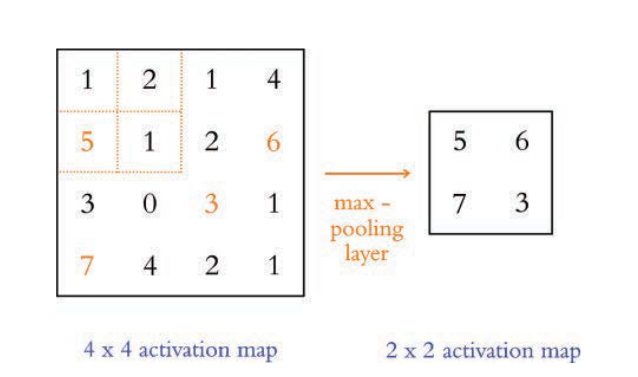
\includegraphics[width=\linewidth]{rys/max-polling.png}
		\caption{Max polling}
		\zrodlo{\cite{illustrated}}
		\label{fig:max-polling}
	\end{figure}
	
\section{Czym jest autoenkoder}

	\textbf{Autoenkoder} (czasem także nazywany autokoderem, z ang. \textit{autoencoder}, \textit{auto-encoder}) jest specjalnym typem sieci neuronowej, która jest przeznaczona głównie do kodowania danych wejściowych do skompresowanej i znaczącej reprezentacji, a następnie dekodowania ich z powrotem w taki sposób, aby zrekonstruowane dane były jak najbardziej podobne do oryginalnych \cite{bank}. Autoenkodery uczą się gęstych reprezentacji danych, tzw. reprezentacji ukrytych (ang. \emph{latent representations}) lub kodowań (ang. \emph{codings}) bez jakiejkolwiek formy nadzorowania (tzn. zbiór danych nie zawiera etykiet). Wyjściowe kodowania zazwyczaj mają mniejszą wymiarowość od danych wejściowych, dzięki czemu autoenkodery mogą z powodzeniem służyć do redukcji wymiarowości. Mają też zastosowanie w \textbf{modelach generatywnych} (ang. \emph{generative models}), które potrafią losowo generować nowe dane przypominające zbiór uczący. Jeszcze lepszej jakości dane można uzyskać przy użyciu \textbf{generatywnych sieci przeciwstawnych}, czyli GAN (ang. \textit{Generative Adversial Networks}). Sieci GAN są często stosowane w zadaniach zwiększania rozdzielczości obrazu, koloryzowania, rozbudowanego edytowania zdjęć, przekształcania prostych szkiców w realistyczne obrazy, dogenerowywania danych służących do uczenia innych modeli, generowania innych typów danych np. tekstowych, dźwiękowych, itd. \cite{geron}.


(Chapter 14 Autoencoders \cite{goodfellow})

An autoencoder is a neural network that is trained to attempt to copy its input
to its output. Internally, it has a hidden layer h that describes a code used to
represent the input. The network may be viewed as consisting of two parts: an
encoder function h = f (x) and a decoder that produces a reconstruction r = g(h).
This architecture is presented in figure 14.1 . If an autoencoder succeeds in simply
learning to set g(f (x)) = x everywhere, then it is not especially useful. Instead,
autoencoders are designed to be unable to learn to copy perfectly. Usually they are
restricted in ways that allow them to copy only approximately, and to copy only
input that resembles the training data. Because the model is forced to prioritize
which aspects of the input should be copied, it often learns useful properties of the
data.


\begin{figure}[!h]
	\centering
	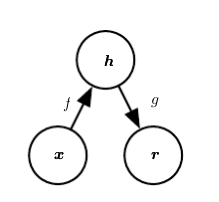
\includegraphics[width=6cm]{rys/autoencoder_structure.png}
	\caption{The general structure of an autoencoder, mapping an input x to an output
		(called reconstruction) r through an internal representation or code h. The autoencoder
		has two components: the encoder f (mapping x to h) and the decoder g (mapping h
		to r ).}
	\zrodlo{\cite{goodfellow}}
	\label{fig:autoencoder_structue}
\end{figure}

\section{Rodzaje autoenkoderów}

Rodzaje autoenkoderów:

- niedopełniony (undercomplete)

- stosowy (stacked) lub inaczej głęboki (deep)

- splotowy (convolutional)

- rekurencyjny (recurrent)

- odszumiający (stacked denoising)

- rzadki (sparse)

- wariancyjny (variational)



\subsection{Autoenkodery niedopełnione}

\cite{goodfellow}

Copying the input to the output may sound useless, but we are typically not
interested in the output of the decoder. Instead, we hope that training the
autoencoder to perform the input copying task will result in h taking on useful
properties.
One way to obtain useful features from the autoencoder is to constrain h to
have a smaller dimension than x. An autoencoder whose code dimension is less
than the input dimension is called undercomplete. Learning an undercomplete
representation forces the autoencoder to capture the most salient features of the
training data.

The learning process is described simply as minimizing a loss function
$$L(x, g(f(x)))$$
where L is a loss function penalizing g(f(x)) for being dissimilar from x, such as
the mean squared error.
When the decoder is linear and L is the mean squared error, an undercomplete
autoencoder learns to span the same subspace as PCA.

\subsection{Autoenkodery stosowe}

(kopiowane z Gerona:)

Autokodery, podobnie jak w przypadku innych rodzajów sieci neuronowych, również mogą mieć
wiele warstw ukrytych. W takiej sytuacji są one nazywane autokoderami stosowymi (ang. stacked
autoencoders) lub głębokimi (ang. deep autoencoders). Kolejne warstwy ukryte pozwalają autokode-
rowi uczyć się bardziej skomplikowanych kodowań. Jednak musimy uważać, aby nie stworzyć
zbyt potężnego modelu. Wyobraź sobie tak wydajny autokoder, że nauczyłby się rzutować każdy
przykład wejściowy do postaci dowolnej pojedynczej liczby (a dekoder uczyłby się odwrotnego rzuto-
wania). Oczywiście taki autokoder potrafiłby doskonale rekonstruować dane uczące, ale w trakcie
tego procesu nie nauczy się żadnej przydatnej reprezentacji danych (i raczej nie będzie w stanie dobrze
generalizować przewidywań na nowe próbki).
Architektura autokodera stosowego najczęściej jest symetryczna względem centralnej warstwy ukrytej
(kodowania). Najprościej mówiąc, przypomina ona kanapkę. Na przykład autokoder klasyfikujący
obrazy MNIST (zbiór ten został opisany w rozdziale 3.) może zawierać 784 wejścia, po których nastę-
puje stuneuronowa warstwa ukryta, następnie środkowa warstwa ukryta zawierająca 30 jednostek,
a po niej kolejna stuneuronowa warstwa ukryta przechodząca w warstwę wyjściową mającą 784 wyj-
ścia.



\chapter{Przykłady zastosowań autoenkoderów}

\section{Analiza PCA za pomocą autoenkodera niedopełnionego}

Jeśli autoenkoder korzysta jedynie z liniowych funkcji aktywacji, a funkcją kosztu jest  błąd średniokwadratowy (MSE), to będzie on przeprowadzał analizę składowych głównych PCA \cite{geron}. Na rysunku \ref{fig:PCA-kod} widoczny jest kod w języku Python służący do utworzenia takiego autoenkodera, który przeprowadzi analizę PCA na zbiorze trójwymiarowym, rzutując go na przestrzeń dwuwymiarową. Można zauważyć podział autoenkodera na dwie części - enkoder i dekoder. Enkoder przyjmuje dane wejściowe o wymiarze 3, a na wyjściu pojawiają się dane dwuwymiarowe. W przypadku dekodera jest odwrotnie - dane na wejściu są dwuwymiarowe, a na wyjściu trójwymiarowe. Obydwie części są modelami sekwencyjnymi z jedną warstwą gęstą, a cały autoenkoder jest modelem sekwencyjnym, w którym po enkoderze występuje dekoder.

\begin{figure}[!h]
	\centering
	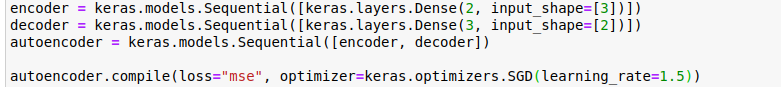
\includegraphics[width=\linewidth]{rys/autoenkoder_PCA_kod.png}
	\caption{Tworzenie autoenkodera niedopełnionego przeprowadzającego PCA}
	\zrodlo{Opracowanie własne na podstawie \cite{geron}}
	\label{fig:PCA-kod}
\end{figure}

\begin{figure}[!h]
	\centering
	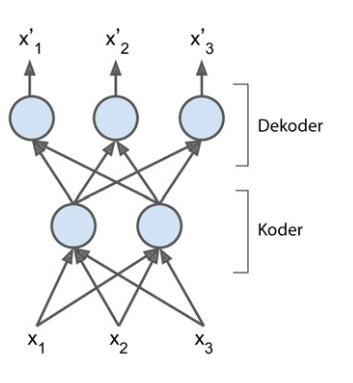
\includegraphics[width=7cm]{rys/ae_undercomplete.png}
	\caption{Architektura autoenkodera niedopełnionego}
	\zrodlo{\cite{geron}}
	\label{fig:ae-undercomplete}
\end{figure}

\newpage

Opisany autoenkoder zostanie wyuczony na wygenerowanym zbiorze trójwymiarowych danych. Warto zwrócić uwagę, że zbiór uczący stanowi jednocześnie dane wejściowe i dane docelowe. Po wytrenowaniu modelu, używamy enkodera do zakodowania danych wejściowych, czyli do zrzutowania ich na przestrzeń dwuwymiarową. Na rysunku \ref{fig:PCA-3d} zaprezentowany jest trójwymiarowy zbiór danych. Rysunek \ref{fig:PCA-2d} przedstawia wynik działania autoenkodera, a więc dane zrzutowane na przestrzeń 2D. Z kolei na rysunku \ref{fig:PCA-zwykle} widoczne jest rzutowanie uzyskane przy użyciu ,,zwykłego'' algorytmu PCA. Na podstawie tych wykresów można stwierdzić, że rzutowanie uzyskane przy pomocy autoenkodera oraz PCA jest takie samo, jedynie układ współrzędnych jest odwrócony o 180 stopni.

\newpage

\begin{figure}[!h]
	\centering
	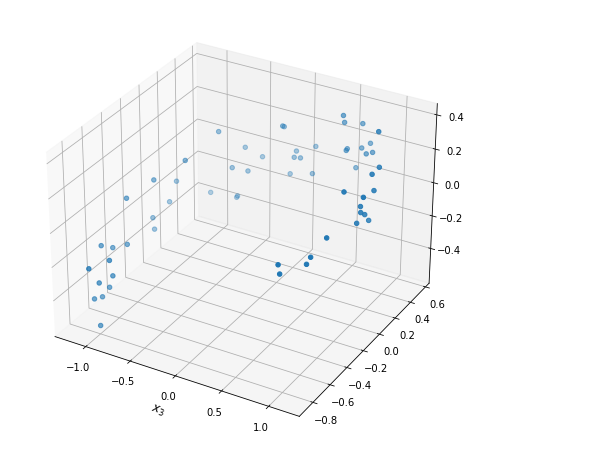
\includegraphics[width=10cm]{rys/pca3d_dane.png}
	\caption{Wygenerowane dane trójwymiarowe}
	\zrodlo{Opracowanie własne na podstawie \cite{geron}}
	\label{fig:PCA-3d}
\end{figure}


\begin{figure}[!h]
	\centering
	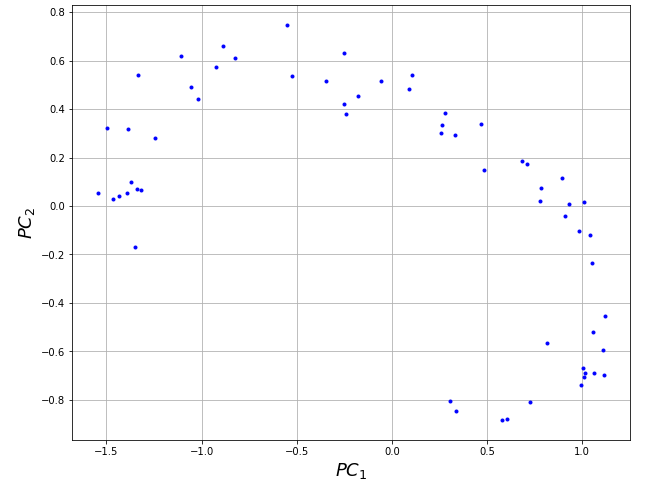
\includegraphics[width=10cm]{rys/pca2d_dane.png}
	\caption{Rzutowanie dwuwymiarowe przy użyciu autoenkodera, zachowujące maksymalną wariancję}
	\zrodlo{Opracowanie własne na podstawie \cite{geron}}
	\label{fig:PCA-2d}
\end{figure}

\newpage

\begin{figure}[!h]
	\centering
	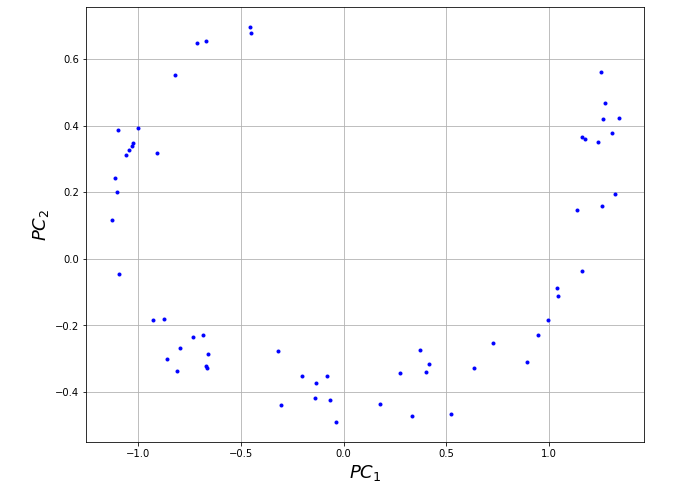
\includegraphics[width=10cm]{rys/pca_zwykle.png}
	\caption{Rzutowanie dwuwymiarowe przy użyciu PCA, zachowujące maksymalną wariancję}
	\zrodlo{Opracowanie własne na podstawie \cite{geron}}
	\label{fig:PCA-zwykle}
\end{figure}

\begin{figure}[!h]
	\centering
	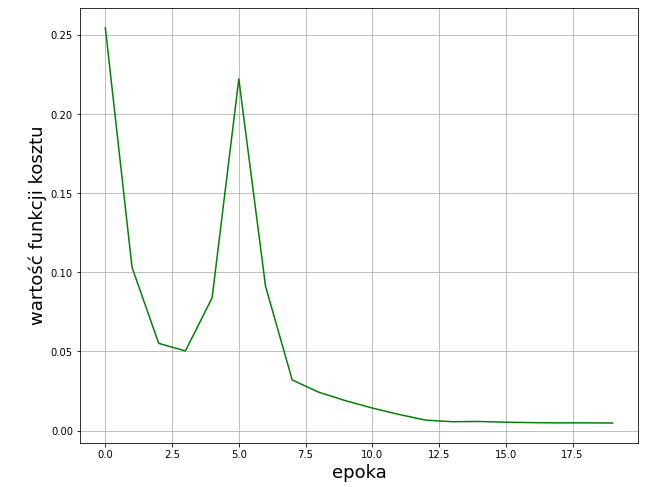
\includegraphics[width=10cm]{rys/ae_undercomplete_loss.png}
	\caption{Wartość funkcji straty w kolejnych epokach podczas uczenia modelu}
	\zrodlo{Opracowanie własne}
	\label{fig:undercomplete-loss}
\end{figure}

\section{Kolejny przykład}


\chapter*{Podsumowanie i~wnioski}


\begin{thebibliography}{99}

\bibitem{aggarwal} Aggarwal, C. C. (2018).\emph{ Neural Networks and Deep Learning}, Springer International Publishing

\bibitem{bank} Bank D., Koenigstein N., Giryes R. (2021), \emph{Autoencoders}, arXiv:2003.05991v2

\bibitem{chollet} Chollet F., Allaire J. J. (2019) \emph{Deep Learning. Praca z językiem R i biblioteką Keras}, Helion SA

\bibitem{edureka} Edureka, Autoencoders Tutorial. Autoencoders in Deep Learning. Tensorflow Training \url{https://www.youtube.com/watch?v=nTt_ajul8NY} 

\bibitem{ertel} Ertel W. (2017) \emph{Introduction to Artificial Intelligence. Second Edition}, Springer International Publishing

\bibitem{geron} G\'eron A. (2020) \emph{Uczenie maszynowe z użyciem Scikit-Learn i TensorFlow. Wydanie II}, Helion SA

\bibitem{goodfellow} Goodfellow I., Bengio Y., Courville A. (2018), \emph{Deep Learning. Systemy uczące się}, PWN, Warszawa 

\bibitem{illustrated} Krohn J., Beyleveld G., Bassens A., \emph{Uczenie głębokie i sztuczna inteligencja. Interaktywny przewodnik ilustrowany}, Helion 2022

\bibitem{osinga} Osinga D. (2019) \emph{Deep Learning. Receptury}, Helion SA

\bibitem{skansi} Skansi S. (2018) \emph{Introduction to Deep Learning. From Logical Calculus to Artificial Intelligence}, Springer International Publishing


\end{thebibliography}



\listoffigures

\listoftables


\chapter*{Załączniki}
\begin{enumerate}
%\item Oświadczenie o oryginalności pracy i możliwości jej wykorzystania. 
%\item Opinia promotora na temat oryginalności pracy oraz w~sprawie dopuszczenia do obrony pracy dyplomowej.
%\item Potwierdzenie analizy antyplagiatowej.
\item Płyta CD z niniejszą pracą w wersji elektronicznej.
\end{enumerate}




\chapter*{Streszczenie (Summary)}

\bigskip
\bigskip

\begin{center}
  \textbf{\tytul}
\end{center}



\bigskip

\begin{center}
  \textbf{\textit{\tytulangielski}}
\end{center}



\selecthyphenation{english}
{\it

}

\end{document}

